\documentclass{article}

\usepackage{amsmath}
\usepackage{amssymb}
\usepackage{fancyhdr}
\usepackage{graphicx}
\usepackage{epstopdf}
\usepackage[top=1in,bottom=1in,right=1.25in,left=1.25in]{geometry}
\usepackage[]{algorithm2e}
\usepackage{tikz}

% For the finite state machine
\usetikzlibrary{arrows,automata}

% Header Settings 
\pagestyle{fancy}
\lhead{Eric Jalbert - 0712946}
\rhead{MATH 6182 - Final Project}
\cfoot{\thepage}
\renewcommand{\headrulewidth}{0.4pt}
\renewcommand{\footrulewidth}{0.4pt}

\graphicspath{{./},{Figures/}}

\begin{document}
\section*{Overview}
%Explain what the experiment is and why we are doing it.
%   Which features of evolutionary computation are under examination,
%   How are we examining them,
%   What do we hope to find out.
The idea for my final project is to use the ideas from evolutinary algorithms to create music. Mainly this will be treated as a proof-of-concept. The different effect mutations and population size has on the fitness of the songs will be analysed. The efficiency of using evolutionary algorithms to generate music for human enjoyability will also be explored. This will be done though the enjoyability of listening to the songs; since this is a proof-of-concept project, this will be sufficient. 

\section*{Methods}
%Describe the methods you are using
%   Give a description, possibly pseudo-code, for the algorithm(s) used
%   State the source of you code (instructor, self, help from who),
%   State the number and type of runs of the code you made

\subsection*{Representation of a Song}
  To work with evolutationary algorithms and fitness functions, a new way of representing songs had to be created. This was done using the idea of bitwise storage of information. Figure \ref{fig:bitRepresentation} shows which bits are allocated to each piece of information. Each note needs a track, channel, volume, duration, and pitch. 
  
  Track has a value from 0 to 15 and channel has a value from 1 to 16, thus can each be represented by 4 bits. Volume is any integer value to represent the loudness of the notes. It can be changed at any note, and effects every note after it. Retricted to values from 0 to 127 here for sake of simplicity. Duration can be any number of values, but for the sake of easy implementation, it is retricted to multiples of $1/8$ notes, going from $1/8$ a beat to $4$ beats and thus only needs 5 bits; implemented with 8 bits so that more duration possibilities can be added at a later date. Pitch can be any note in the range of possible values, here the range of a standard piano is used, which is 88 possible pitches spanning the frequency range $27.5 Hz$, A0, to $4186 Hz$, C8. Now that notes can be represented by a 32 bit integer, a series of these integers makes up a song. 

\begin{figure}[h!tb]
\begin{center}
    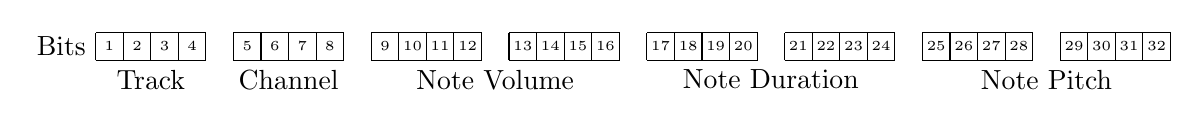
\begin{tikzpicture}[scale=0.35]
        \draw (0,0) -- (4,0) -- (4,1) -- (0,1);
        \draw (5,0) -- (9,0) -- (9,1) -- (5,1);
        \draw (10,0) -- (14,0) -- (14,1) -- (10,1);
        \draw (15,0) -- (19,0) -- (19,1) -- (15,1);
        \draw (20,0) -- (24,0) -- (24,1) -- (20,1);
        \draw (25,0) -- (29,0) -- (29,1) -- (25,1);
        \draw (30,0) -- (34,0) -- (34,1) -- (30,1);
        \draw (35,0) -- (39,0) -- (39,1) -- (35,1);
        \foreach \i in {0,...,39}{\draw (\i,0) -- (\i,1);}
        \foreach \i in {29,...,32}{\node at (\i+6.5,0.5) {\tiny{\i}};}
        \foreach \i in {25,...,28}{\node at (\i+5.5,0.5) {\tiny\i};}
        \foreach \i in {21,...,24}{\node at (\i+4.5,0.5) {\tiny\i};}
        \foreach \i in {17,...,20}{\node at (\i+3.5,0.5) {\tiny\i};}
        \foreach \i in {13,...,16}{\node at (\i+2.5,0.5) {\tiny\i};}
        \foreach \i in {9,...,12}{\node at (\i+1.5,0.5) {\tiny\i};}
        \foreach \i in {5,...,8}{\node at (\i+0.5,0.5) {\tiny\i};}
        \foreach \i in {1,...,4}{\node at (\i-0.5,0.5) {\tiny\i};}
        \node [left] at (0,0.5) {Bits};
        \node [below] at (2,0) {Track};
        \node [below] at (7,0) {Channel};
        \node [below] at (14.5,0) {Note Volume};
        \node [below] at (24.5,0) {Note Duration};
        \node [below] at (34.5,0) {Note Pitch};
    \end{tikzpicture}
    \caption{Representation of a single note using 32 bits}
    \label{fig:bitRepresentation}
\end{center}
\end{figure}


\subsection*{Evolving a Song}
Algorithm \ref{alg:evolveSong} shows the overview for how the songs are evolved. Each step is explained in further detail in the following subsections.

\begin{algorithm}[h]
\dontprintsemicolon
\KwData{runs = 10; popSize = 32; genLength = 500; bestInGen = 150}
\Begin
{
  \SetLine
  \For{each iterate in \textbf{runs}}
  {
    Initialize a new population of size \textit{\textbf{popSize}}\;
    \For{each generation in \textbf{genLength}}
    {
      Compute the fitness of each member\;
      Store the top \textit{\textbf{bestInGen}} members\;
      Use mutations to create members until there are \textit{\textbf{popSize}} members\;
    }
    Convert the top \textit{\textbf{bestInGen}} members into MP3's
  }
}
\caption{Algorithm for evolving songs; created by Eric Jalbert, implemented in Python.}
\label{alg:evolveSong}
\end{algorithm}

\subsubsection*{Initialize Population}
The initialization of the population is depicted in Algorithm \ref{alg:initPop}. The channel number and volume are hard coded to simplify the evolutions. Also, the real purpose of channel number is not known at this point. 

\begin{algorithm}[h]
\dontprintsemicolon
\KwData{numTracks = 2; numNotes = 100}
\Begin
{
  \SetLine
  Set channel number to 0\;
  Set volumn to 127 always\;
  \For{each \textbf{i} in \textbf{numTracks}}
  {
    Set track number to \textbf{\textit{i}}\; 
    \For{each of the \textbf{numNotes} notes}
    {
        Randomize a duration and pitch\;
        Write the note to file\;
    }
  }
}
\caption{Algorithm for initializing the population; created by Eric Jalbert, implemented in Python.}
\label{alg:initPop}
\end{algorithm}

\subsubsection*{Computing Fitness}
The algorithm for computing the fitness is described in Algorithm \ref{alg:fitness}. It is based on the compilation of multiple fitness functions that each combine into a robust fitness function. These can be taken externally as arguments to the program so that different features in a song can be added. Extra control is given by the \textbf{\textit{fitWeight}} of the function, creating a weighted average of each fitness function. 

\begin{algorithm}[h]
\dontprintsemicolon
\KwData{numFuncs = 2}
\Begin
{
  \SetLine
  \For{each fitness function of \textbf{numFuncs}}
  {
    Check song against fitness function\;
    Multiple the fitness by \textbf{\textit{fitWeight}}\;
    Add this value to \textbf{\textit{totalFitness}}\;
  }
  Return \textbf{\textit{totalFitness}} as the fitness of song\;
}
\caption{Algorithm for computing the fitness of a song; created by Eric Jalbert, implemented in Python.}
\label{alg:fitness}
\end{algorithm}


\subsubsection*{Mutations}
The mutations for this follow algorithm \ref{alg:mutations}. The crossover is done by taking a random section of notes from one parent and then replacing a random section of notes in the other parent. Here the size of each section is forced to be equal. This could probably be changed so as to encourage more dynamic members in the population, but this was avoided here for simplicity.

\begin{algorithm}[h]
\dontprintsemicolon
\KwData{bestInGen = 5; mnm = 3; popSize = 32}
\Begin
{
  \SetLine
  Store top \textit{\textbf{bestInGen}} members\;
  \While{there are less then \textbf{popSize} members}
  {
    Pick two randoms from the \textit{\textbf{bestInGen}} members\; 
    Create child by crossing over between two members\;
    Do \textit{\textbf{mnm}} single point mutations on child\;
    Add child to population\;
  }
  Return new population\;
}
\caption{Algorithm for mutating the population; created by Eric Jalbert, implemented in Python.}
\label{alg:mutations}
\end{algorithm}


\subsubsection*{Converting to MP3}
The conversion of a string of bits into an MP3 is described in algorithm \ref{alg:convert}. The main thing here is the fact that the series of 32-bit values actually gets converted to a MIDI file first, which can easily be converted to MP3. 

\begin{algorithm}[h]
\dontprintsemicolon
\KwData{songFileName; bitFileName}
\Begin
{
  \SetLine
  Write preamble for conversion to \textit{\textbf{songFileName}}\;
  \For{each note in \textbf{bitFileName}}
  {
    Convert 32-bit into a single note\;
    Write note to \textit{\textbf{songFileName}}\;
  }
  Write postamble for conversion to \textit{\textbf{songFileName}}\;
  Convert \textit{\textbf{songFileName}} to MIDI file\;
  Convert MIDI file to MP3\;
}
\caption{Algorithm for converting a series of 32 bits into an MP3; created by Eric Jalbert, implemented in Python.}
\label{alg:convert}
\end{algorithm}


\section*{Results}
%Clearly describe you results.
%   Give a summary, probably table(s) or graph(s), of the results you obtained. 
%   Present those results as clearly as possible.
%   Where possible, support your results with statistics.
%   Use statistics to determine the significance of your results.
The results of my work are extremely preliminary. Still, the effect of typical evoluationary parameters had a bit of an effect on the resulting song and fitness. The change in average and maximum fitness for different parameter values can be seen in Figure \ref{fig:paramChange}. 

\begin{figure}[h]
    \begin{center}
        \begin{tabular}{c c}
        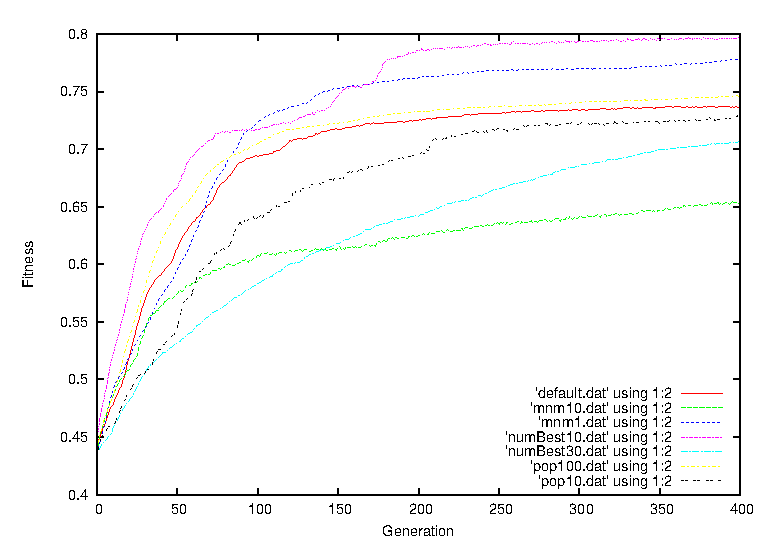
\includegraphics[scale=0.55]{paramChangeAvg.eps} &
        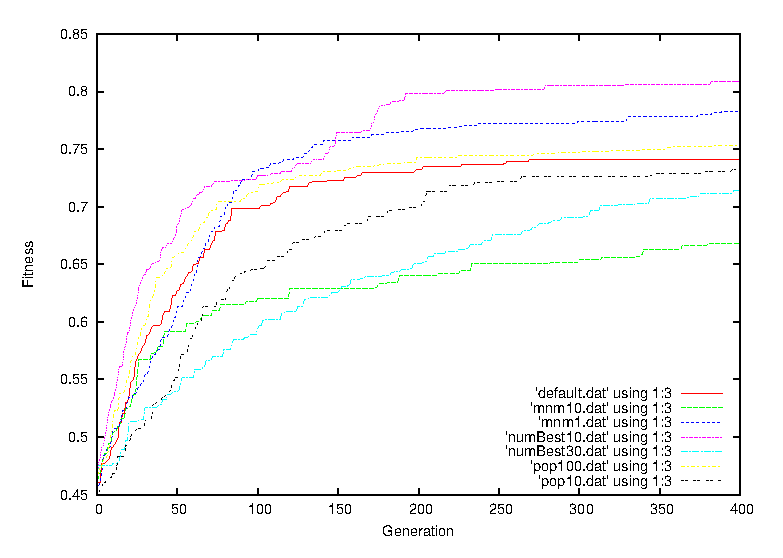
\includegraphics[scale=0.55]{paramChangeMax.eps} \\
        (a) & (b) 
        \end{tabular}
        \caption{Different parameter settings gives different (a) average fitness and (b) maximum fitness. 'mnmXX' is the number of point mutations; 'numBestXX' is the number of top songs stored each generations; 'popXXX' is the population size.}
        \label{fig:paramChange}
    \end{center}
\end{figure}

The variabilty of the fitness between runs was examined in Figure \ref{fig:betweenRuns}. This was done so that variability could be ruled out as an explaination of the results in Figure \ref{fig:paramChange}.

\begin{figure}[h]
    \begin{center}
        \begin{tabular}{c c}
        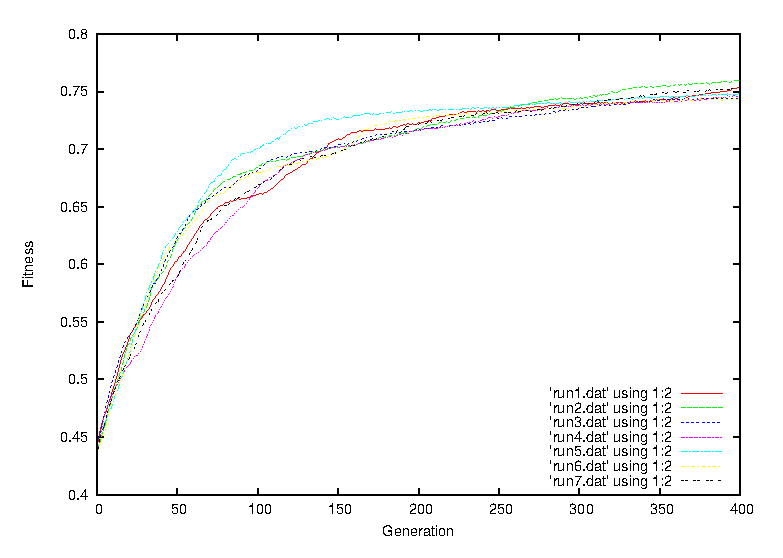
\includegraphics[scale=0.55]{betweenRunAvg.eps} &
        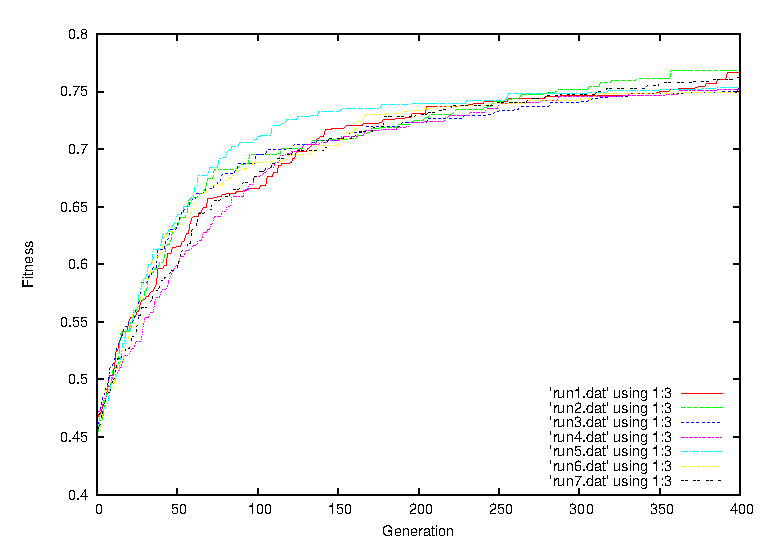
\includegraphics[scale=0.55]{betweenRunMax.eps} \\
        (a) & (b) 
        \end{tabular}
        \caption{Different runs give similar (a) average fitness and (b) maximum fitness}
        \label{fig:betweenRuns}
    \end{center}
\end{figure}

The resulting songs are not completely enjoyable. But the songs with high fitness tend towards a repetative pattern that is bearable. Listen to $repeatative.mp3$. They are also, understandably, dependent on the choice of fitness functions.



\section*{Conclusions and Discussion}
%Explain what happened and why you think it happened.
%    State what significance the results had in terms of the test environment and the features of evolutionary computation under investigation
%    State problems you encountered in gathering data.
%    Explain your results logically and with support, include alternate explanations if you see them.

The results from Figure \ref{fig:paramChange} show that the parameter set does have an effect on the fitness. Mainly that using only one single point mutation and storing a smaller number of top songs per generation is best and that having too many single point mutations and storing too many top songs is bad. These make sense. Because of the nature of the fitness function and how each note needs to work with one another, having too many single point mutations destroys the synergy between notes and lowers the fitness. The storing of a small number of top songs is also sensible. Since the top songs are used as a precursor for the next generation, having a smaller selection forces the children to have sections of notes that have higher fitness. The only issue with this is that the population of songs begin to sound very similar. 

The use of evolutinary algorithms to generate songs appears to work. There are a few issues that need to be sorted out before it becomes efficient though. The variability of the parameter set change the fitness of the population of songs, but this does not effect the enjoyability of the music as much as the choice in fitness function. In fact this choice of fitness function is completely what creates enjoyable music. Because even though a parameter set may give a high fitness in the population, this does not mean much if the high fitness if the result of a fitness function that rewards poor composition of notes. The main issue with this is that choosing the fitness function is a very difficult ordeal. Since to get a song with many different characteristics would require many fitness functions, which would likely lead to contradictory allocations of fitness giving unsatisfactory results. That being said, the songs that have very high fitness tend to be extremly repeatative. This is because the evolutionary algorithm finds the easiest pattern that can repeated to abuse the fitness function and passing into the next generation. This show of repeatative song with high fitness can be heard in $repeatative.mp3$.

Given the constraint of time, there was only so much work that could be done on this implementation. Some future plans that could be done to improve results would be to look into developing a more robust way of having multiple fitness functions. The idea here would be to have a repository of fitness functions, each encouraging a different aspect in the population of songs. At that point, super fitness functions could be made by grouping up the groups. For example, having a fitness function to force songs in C scale, and another to have low pitch notes play arpeggio's could be smaller fitness functions. Together the two fitness functions could, with other fitness functions, make a super fitness function that creates songs in a jazz style. This kind of variability should be possible, just difficult to actually find the right combination of fitness functions to result in what is needed. One major issue with the current implementation is that the fitness function evaluates the song as a whole, where it should instead compute the fitness for each individual track. This would allow each track to take a particular role in the song (bass, melody, harmory, etc.). This would also open the possibility of instrument specific fitness functions. Here the piano instrument was forced for simplicity, but different instruments could be played on each track, with a specific fitness function for each to match with the instruments playing style.

There are many things that can be done to improve on the current implementation of this evoluationary algorithm for generating songs, but it seems promising that it works to a certain degree. 




\end{document}







